%!TEX root = disclosure_game.tex
%Include the descent into chaos bit
\section{Results}
\label{sec:results}


\subsection{Qualitative Trends}
\label{sub:qt_results}

As shown in figure \ref{fig:honest_signals}, all four decision rules were able to reproduce both qualitative trends towards more disclosure as women experience more appointments \citep{Phillips2007}, and a greater tendency towards underreporting of consumption by heavier drinkers \citep{Alvik2006}.  Trends for all four rules are broadly similar, exhibiting a gradual increase across appointments which subsequently levels off. This levelling can in part be explained by the referral results, which show that the majority of drinkers are referred, even with substantial concealment. Referrals continue to occur, in the absence of honest signals, because drinkers are able to achieve a referral by masquerading as higher or lower types, dependent on how their initial beliefs are biased. Despite this the results suggest that a minority of risky drinkers will evade detection altogether, with no notable distinction between heavy and moderate types. Under these parameters, light drinkers always signal honestly and are never referred since there is no perceived advantage in doing so, and the evidence of deceptive signalling is insufficient to outweigh the biased priors of the midwives. 

\begin{figure}[h]
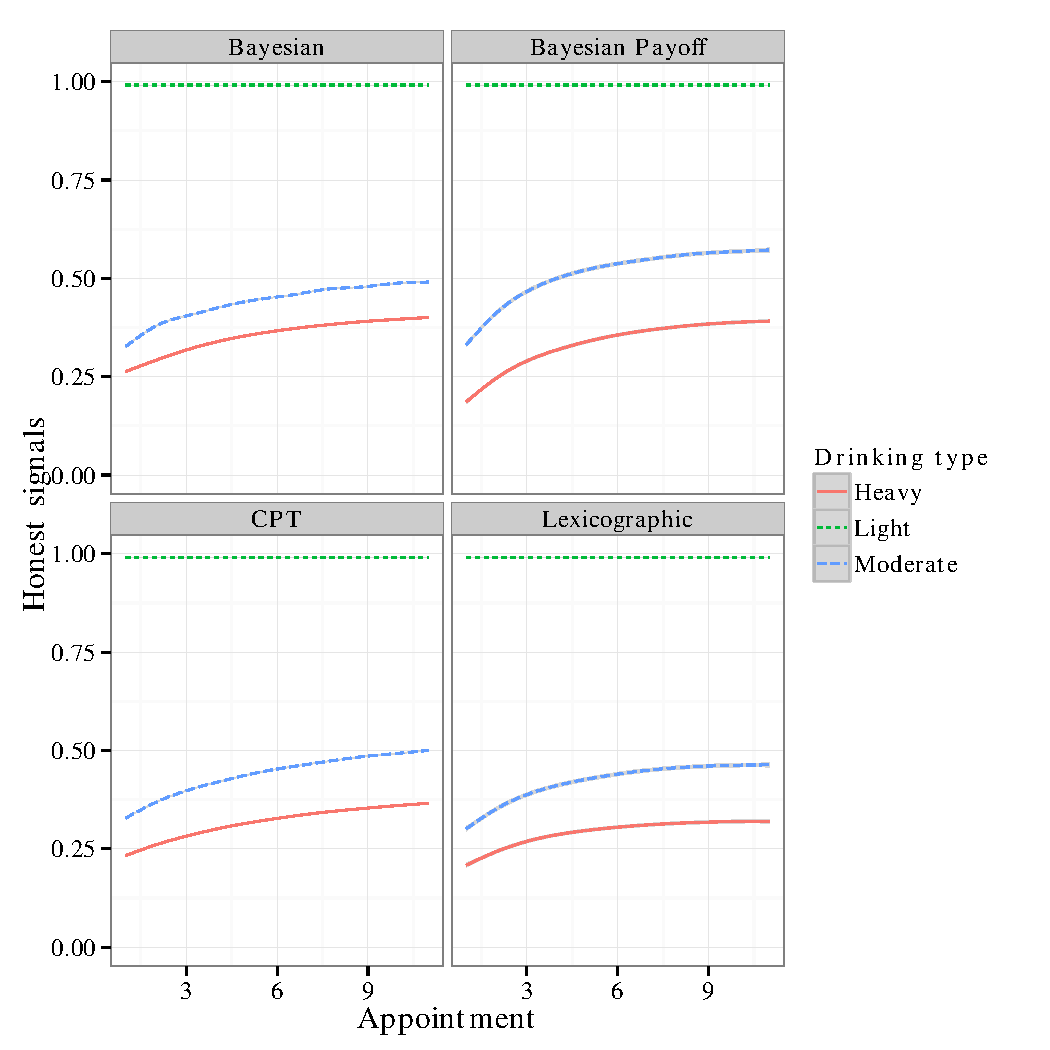
\includegraphics[width=119mm]{figures/honesty_plot}
\caption{Average fraction of population ever signalled honestly after 1000 rounds, mean with 95\% confidence limit over 1000 runs\label{fig:honest_signals}}
\end{figure}

\subsection{Social Learning}
\label{sub:sharing_results}

Introducing social learning amongst women leads the behaviour of the decision rules to diverge markedly. Figure \ref{fig:honest_sharing} shows the proportion of women who have signalled honestly at least once by their final appointment, under four sharing conditions. 

\begin{figure}
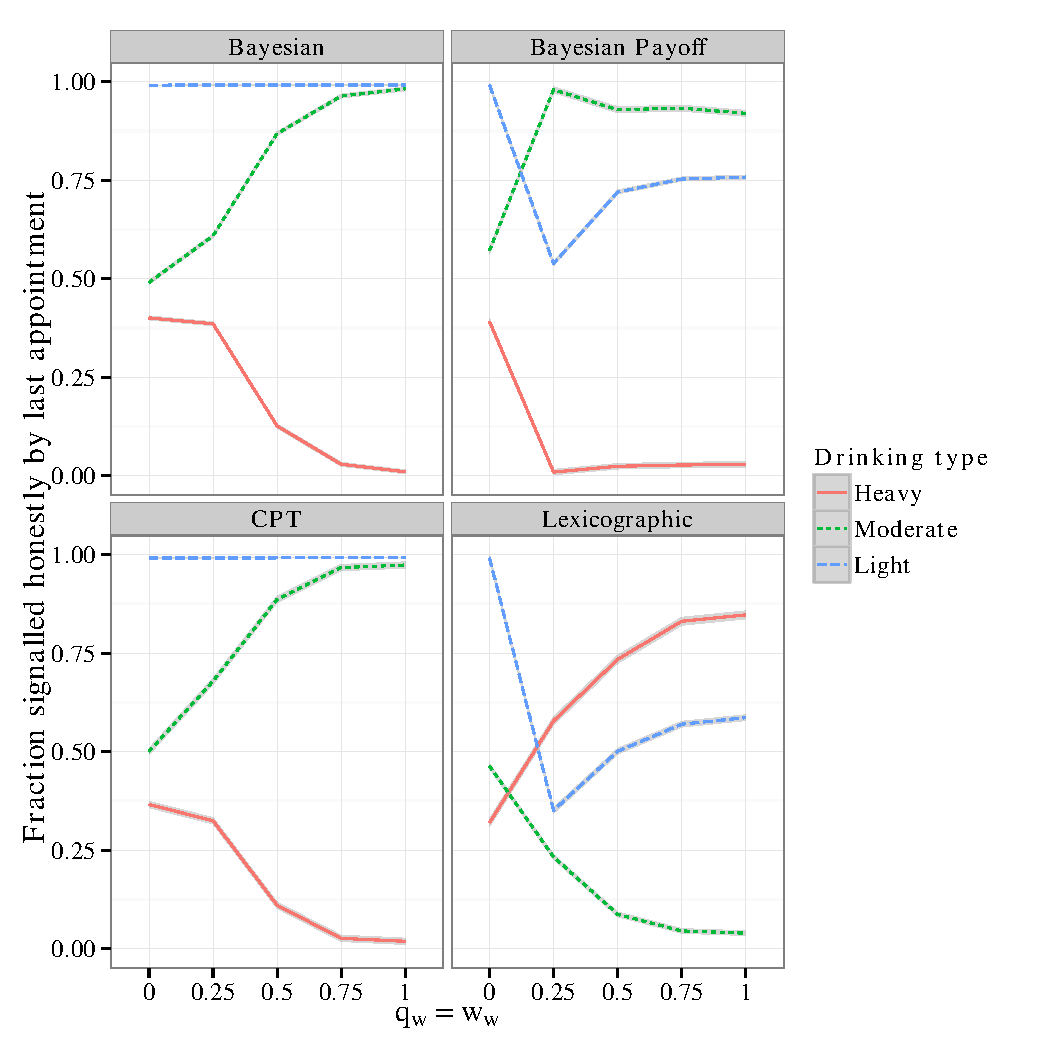
\includegraphics[width=119mm]{figures/honesty_sharing}
\caption{Impact of social learning on trends in honest signalling after 1000 rounds, mean with 95\% confidence interval over 100 runs}
\label{fig:honest_sharing}
\end{figure}

Aside from the lexicographic decision rule, the general tendency is towards less honest signalling by heavy drinkers, which is accompanied by a slight increase in referrals for the Bayesian, and \ac{CPT} rules. For these decision models, this is because social learning exacerbates the existing tendency of heavy drinkers to impersonate moderate drinkers, who behave more honestly as heavy drinkers become less so.

Particularly notable, is the decline in honest signalling by light drinkers visible in both heuristic type rules at the 0.25 level of \(q_{w}\) \& \(w_{w}\), which is associated with an increase in false positives. This arises because of the lack of homophily in social learning, as light drinkers become informed about negative outcomes associated with concealment, despite having nothing to conceal. The relatively high referral rates of drinkers heighten the effect further, because shared information becomes dominated by their experiences. 

The relationship is not, however, entirely straightforward, in that increasing social learning leads to greater variance between runs. A linear model was used to predict the between-runs interquartile range of the average signal sent by moderate drinkers. The predictors used were decision rule, and level of social learning, together with the interaction between the two. The regression results were significant (\(F_{7,12}=25,p<2.9\times10^{-6}\)) with \(R^2=94\%\), and intercept 0.07. The only significant coefficients were for the interaction terms, which were 0.44 (\(p<0.05\)) for the Bayesian payoff rule, and 0.69 (\(p<0.005\)) for the lexicographic. This suggests that social learning, for the heuristic style decision rules introduces considerable uncertainty to the model, which is explored further in the sensitivity analysis below.


\subsection{Sensitivity Analysis}
\label{sub:sa_results}

In this section we present a brief overview of the sensitivity analysis, followed by selected results highlighting the global effect of changes to perceived payoffs and degree of bias towards honesty, as well as social learning within women. The full results for the sensitivity analysis covering all sixteen emulators are available in appendix \ref{app:sensitivity_results}.

For the median signal choice of moderate drinkers, the results of the sensitivity analysis suggest that the proportion of light drinkers has a significant effect for all decision rules, accounting for 10\%, 38\%, 24\%, and 5\% of the variance in output for the Lexicographic, Bayesian Payoff, Bayesian, and \ac{CPT} rules respectively. For the Lexicographic rule, the overwhelming majority of variance in signalling behaviour is reflective of the prevalence of stigmatisation by midwives (44\% \(p_{m}(m)\), 7\% \(p_{l}(m)\), and a further 15\% for their interaction).  The proportions of midwives are also key drivers in group separation, and the between run IQR of both measures for this rule. 

Perhaps surprisingly, variance attributable to social learning between midwives is relatively low, with neither the weight nor probability accounting for more than 5\% of variance in any measure. While there are small contributions to variance in interaction with other parameters (e.g. 4\% to between groups IQR, for the interaction with the proportion of light drinkers under the Bayesian rule), this may suggest that the model is lacking in this area, which we touch on in section \ref{sec:conclusion}.

\begin{figure}[h]
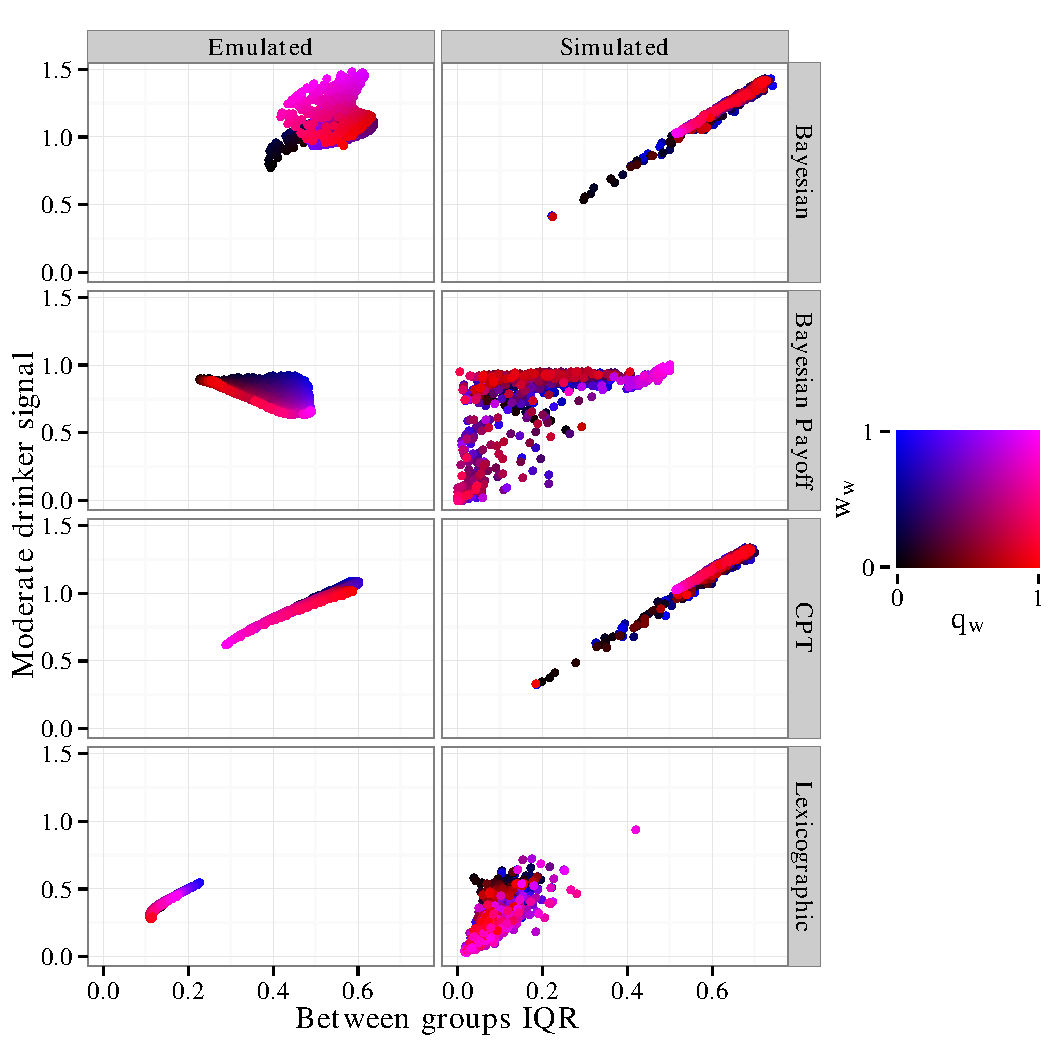
\includegraphics[width=119mm]{figures/sharing_emulated_simulated}
\caption{Median moderate drinker signal vs median between drinking type IQR for all decision rules, with signals coded as 0 = light, 1 = moderate, and 2 = heavy.}
\label{fig:outcome_plots}
\end{figure}

Figure \ref{fig:outcome_plots} gives a qualitative picture of both emulator quality, and the divergent response surfaces of the decision rules in response to variations in social learning parameters. Emulator fit is clearly imperfect, but overall behaviour is qualitatively similar, with both emulated and simulated plots demonstrating separation in outcome space for the decision rules.

\begin{figure}[h]
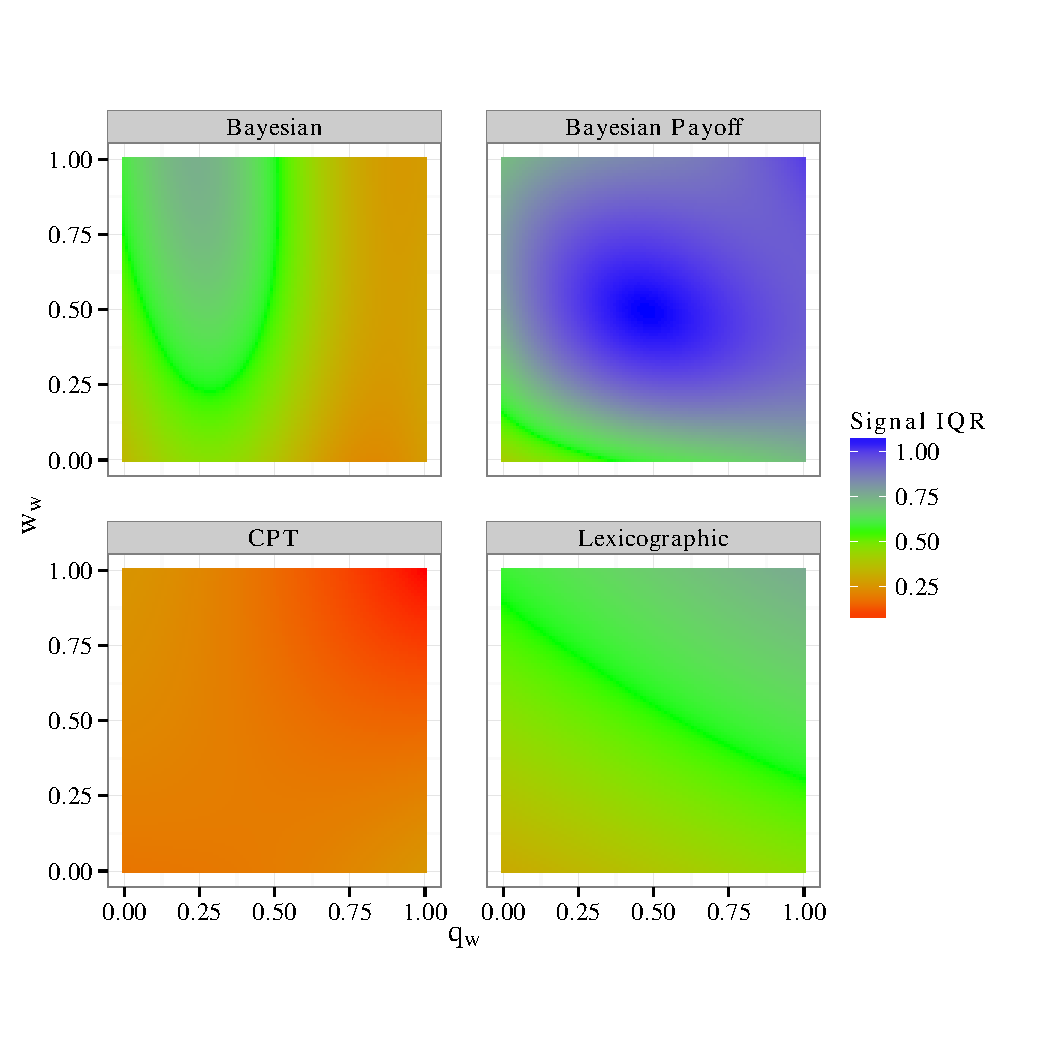
\includegraphics[width=119mm]{figures/unfixed_emu_sig_iqr}
\caption{Emulated moderate drinker signal IQR in response to varying \(q_{w}\), and \(w_{w}\)}
\label{fig:emulated_sharing_iqr}
\end{figure}

Following from the suggestive results for social learning introducing uncertainty (section \ref{sub:sharing_results}), figure \ref{fig:emulated_sharing_iqr} shows emulated points covering the parameter space in high resolution. These plots reflect the increase in uncertainty of outcome shown for the heuristic type rules, which is especially severe for the Bayesian payoff rule. They also suggest that the Bayesian decision rule is less stable under conditions where the weight of shared information is substantially higher than the probability of sharing. This indicates that placing a high weight on information from limited sources leads to greater variability, i.e. what information shared, matters.

For the \ac{CPT}, and Bayesian decision models, the interaction of bias towards honesty, and distinction between payoffs has a significant, and non-linear effect on instability, and separability of groups. Figure \ref{fig:emulated_payoff_group_iqr} shows the effects, and also highlights the tendency towards poor separability of groups for both the heuristic type decision rules. The response surface of the Bayesian payoff rule is slightly more nuanced than the simple Lexicographic rule. Figure \ref{fig:emulated_payoff_group_iqr} shows better separation, close to partial pooling\footnote{Pooling occurs when signallers of different types `pool' their signals, and one adopts the signals of another.} at high payoff distinction, with relatively modest honesty bias, which is reflected by the variance contributions of 11\% and 8\% respectively.  For the more complex rules, the general tendency is towards less pooling for higher values of both, but with pockets where full pooling\footnote{Indicating that all signaller types are using a single signal.} occurs.  The plots also suggest that the sensitivity of the \ac{CPT} rule is marginally greater, which is supported by the significant contribution to variance of close to 15\% for all measures of \(x_{h}\).

\begin{figure}[H]
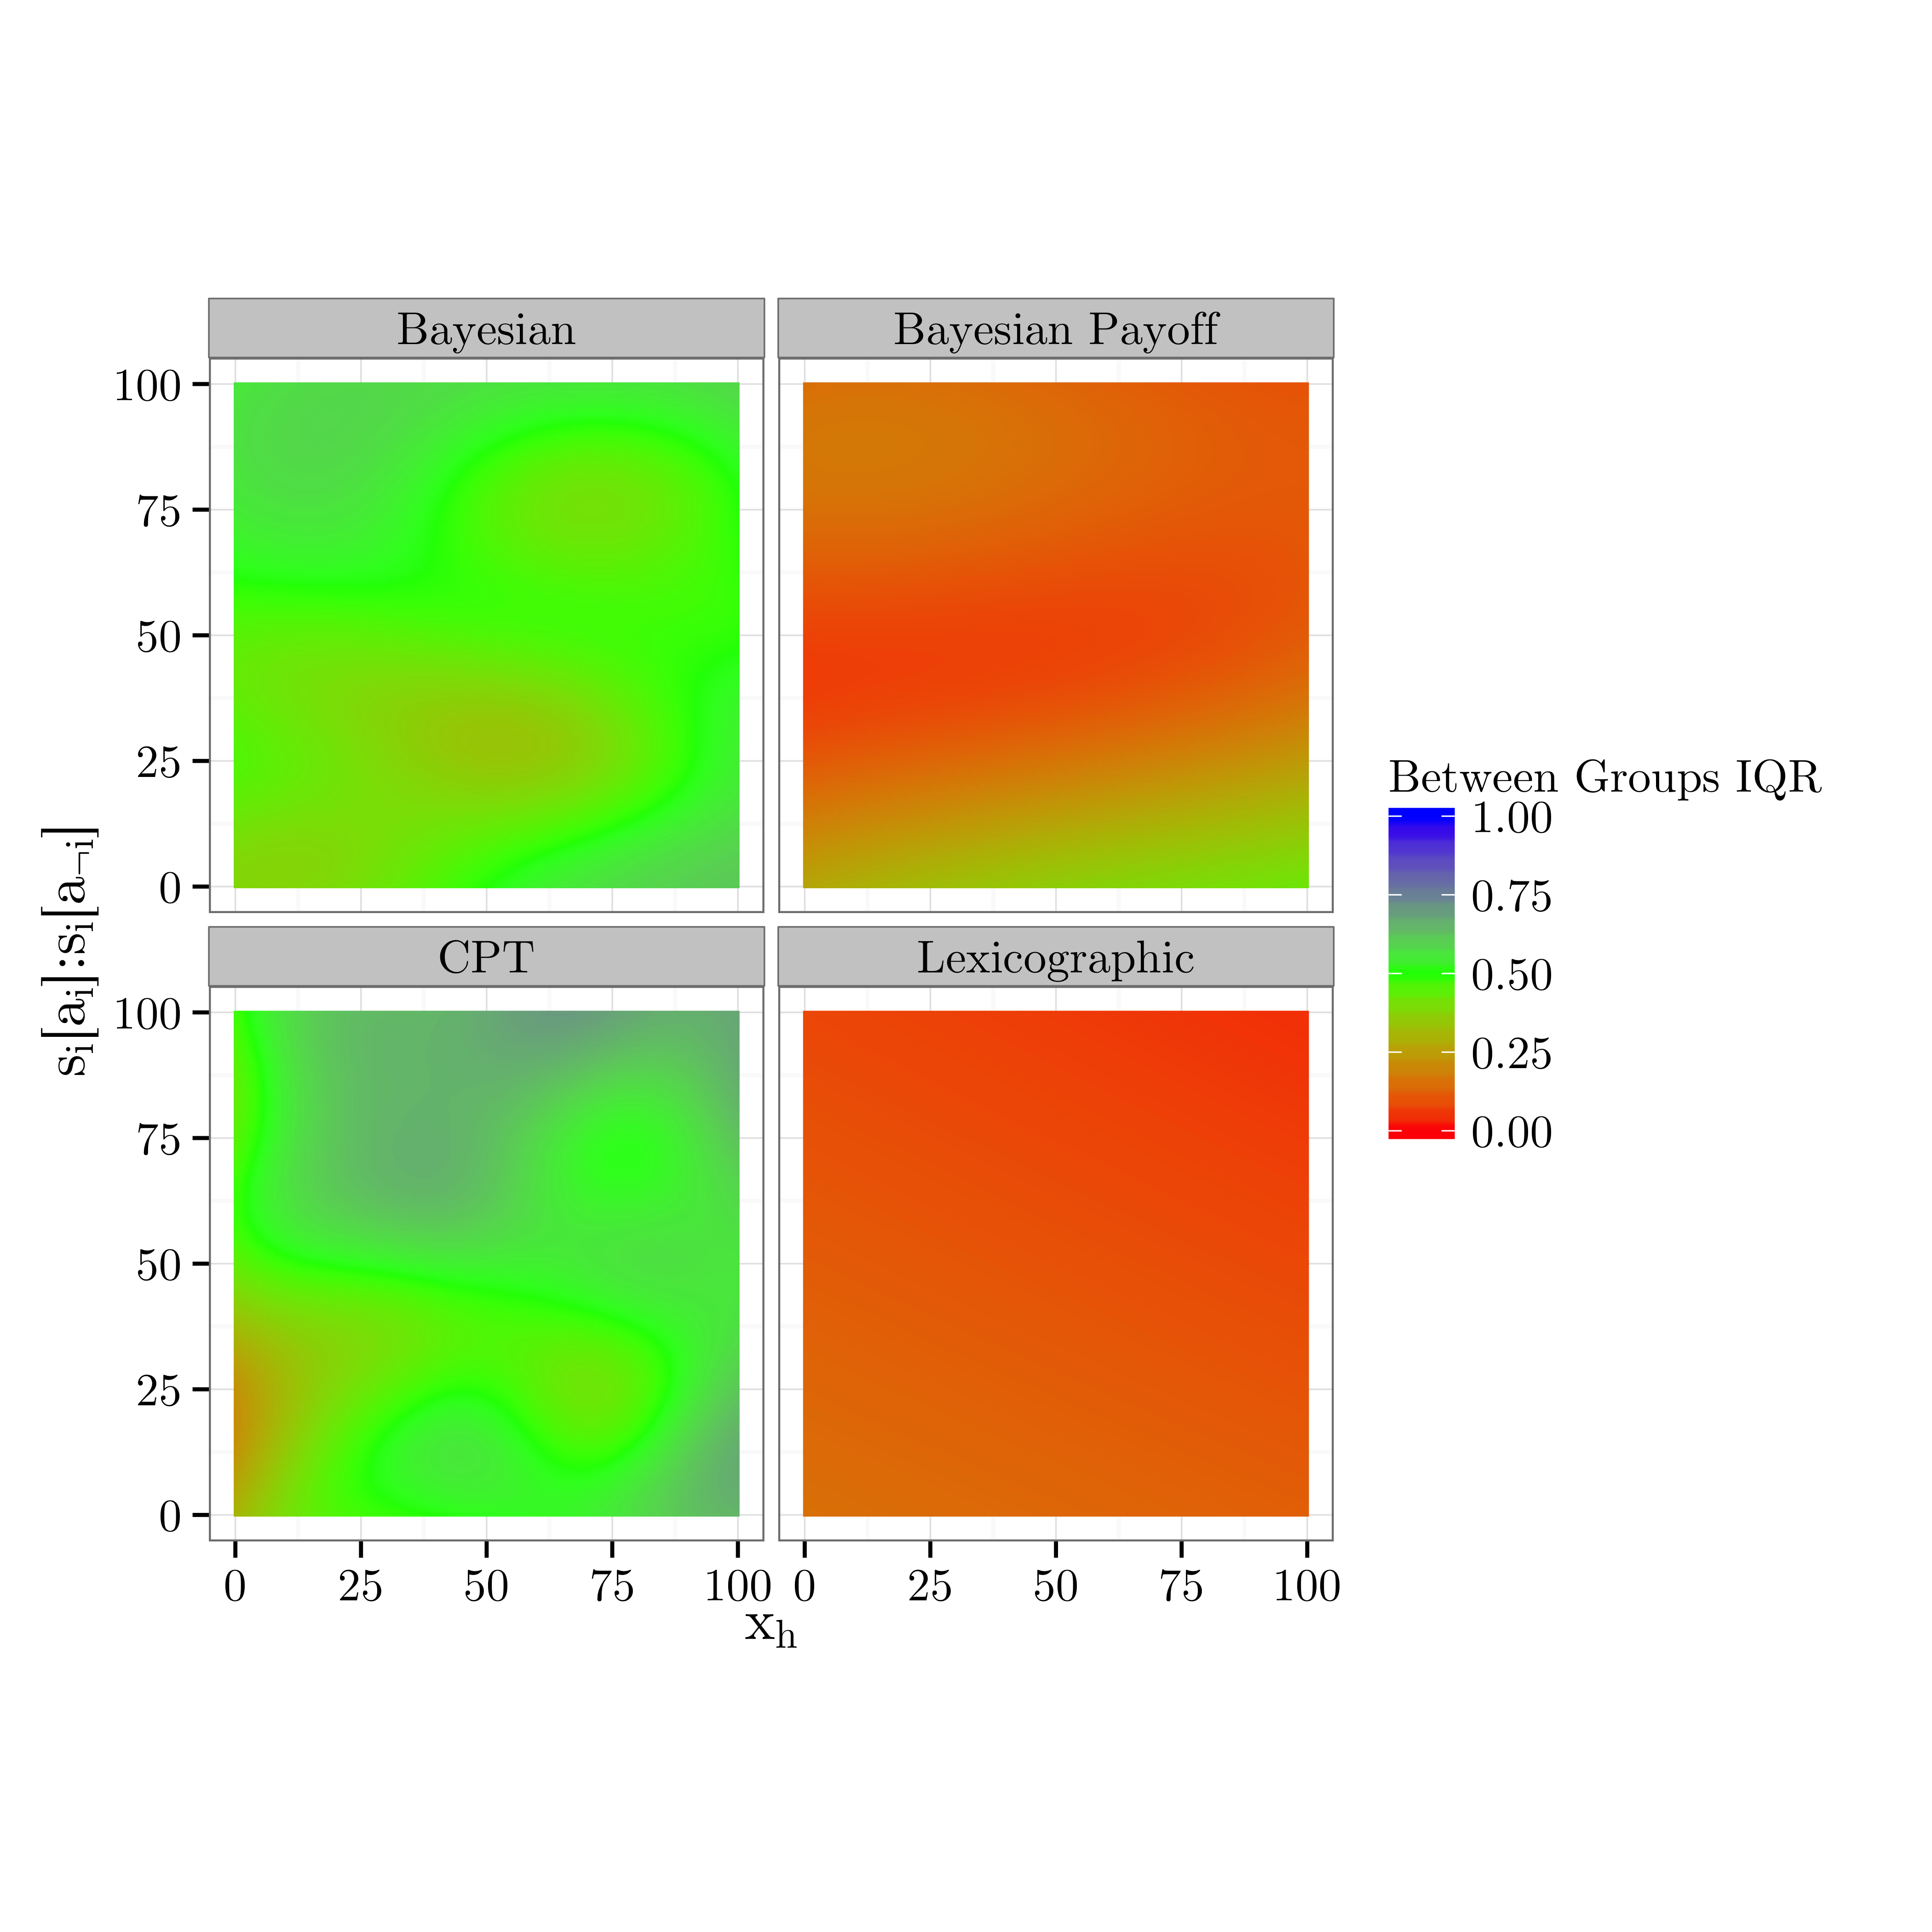
\includegraphics[width=119mm]{figures/unfixed_emu_payoff_honesty_group_iqr}
\caption{Emulated between groups IQR in response to varying \(s_{i}[a_{i}]:s_{i}[a_{\neg i}]\), and \(x_{h}\)}
\label{fig:emulated_payoff_group_iqr}
\end{figure}
